%% Copernicus Publications Manuscript Preparation Template for LaTeX Submissions
%% ---------------------------------
%% This template should be used for copernicus.cls
%% The class file and some style files are bundled in the Copernicus Latex Package, which can be downloaded from the different journal webpages.
%% For further assistance please contact Copernicus Publications at: production@copernicus.org
%% https://publications.copernicus.org/for_authors/manuscript_preparation.html


%% Please use the following documentclass and journal abbreviations for preprints and final revised papers.

%% 2-column papers and preprints
\documentclass[amt, manuscript]{copernicus}



%% Journal abbreviations (please use the same for preprints and final revised papers)


% Advances in Geosciences (adgeo)
% Advances in Radio Science (ars)
% Advances in Science and Research (asr)
% Advances in Statistical Climatology, Meteorology and Oceanography (ascmo)
% Aerosol Research (ar)
% Annales Geophysicae (angeo)
% Archives Animal Breeding (aab)
% Atmospheric Chemistry and Physics (acp)
% Atmospheric Measurement Techniques (amt)
% Biogeosciences (bg)
% Climate of the Past (cp)
% DEUQUA Special Publications (deuquasp)
% Drinking Water Engineering and Science (dwes)
% Earth Surface Dynamics (esurf)
% Earth System Dynamics (esd)
% Earth System Science Data (essd)
% E&G Quaternary Science Journal (egqsj)
% EGUsphere (egusphere) | This is only for EGUsphere preprints submitted without relation to an EGU journal.
% European Journal of Mineralogy (ejm)
% Fossil Record (fr)
% Geochronology (gchron)
% Geographica Helvetica (gh)
% Geoscience Communication (gc)
% Geoscientific Instrumentation, Methods and Data Systems (gi)
% Geoscientific Model Development (gmd)
% History of Geo- and Space Sciences (hgss)
% Hydrology and Earth System Sciences (hess)
% Journal of Bone and Joint Infection (jbji)
% Journal of Micropalaeontology (jm)
% Journal of Sensors and Sensor Systems (jsss)
% Magnetic Resonance (mr)
% Mechanical Sciences (ms)
% Natural Hazards and Earth System Sciences (nhess)
% Nonlinear Processes in Geophysics (npg)
% Ocean Science (os)
% Polarforschung - Journal of the German Society for Polar Research (polf)
% Primate Biology (pb)
% Proceedings of the International Association of Hydrological Sciences (piahs)
% Safety of Nuclear Waste Disposal (sand)
% Scientific Drilling (sd)
% SOIL (soil)
% Solid Earth (se)
% State of the Planet (sp)
% The Cryosphere (tc)
% Weather and Climate Dynamics (wcd)
% Web Ecology (we)
% Wind Energy Science (wes)


%% \usepackage commands included in the copernicus.cls:
%\usepackage[german, english]{babel}
%\usepackage{tabularx}
%\usepackage{cancel}
%\usepackage{multirow}
%\usepackage{supertabular}
%\usepackage{algorithmic}
%\usepackage{algorithm}
%\usepackage{amsthm}
%\usepackage{float}
%\usepackage{subfig}
%\usepackage{rotating}


\begin{document}

\title{Towards Laboratory-level Accuracy in the Field: Spectroscopic Uncertainty in Greenhouse Gas Sensing with Frequency Combs}


 \Author[1]{Newton}{Nguyen}

\Author[]{}{}
\Author[1]{Christian}{Frankenberg}
\Author[2]{Kevin}{Cossel}
\affil[]{Division of Geology and Planetary Science, California Institute of Technology, Pasadena, California, USA}
\affil[]{National Institute of Standards and TEchnology, Boulder, Colorado, USA}

%% The [] brackets identify the author with the corresponding affiliation. 1, 2, 3, etc. should be inserted.

%% If an author is deceased, please mark the respective author name(s) with a dagger, e.g. "\Author[2,$\dag$]{Anton}{Smith}", and add a further "\affil[$\dag$]{deceased, 1 July 2019}".

%% If authors contributed equally, please mark the respective author names with an asterisk, e.g. "\Author[2,*]{Anton}{Smith}" and "\Author[3,*]{Bradley}{Miller}" and add a further affiliation: "\affil[*]{These authors contributed equally to this work.}".


\correspondence{Newton Nguyen (newton@caltech.edu)}

\runningtitle{Spectroscopic Uncertainty}

\runningauthor{Nguyễn et al.}





\received{}
\pubdiscuss{} %% only important for two-stage journals
\revised{}
\accepted{}
\published{}

%% These dates will be inserted by Copernicus Publications during the typesetting process.


\firstpage{1}

\maketitle



\begin{abstract}
Long-term monitoring of long-lived greenhouse gases (ghgs) requires sub-percent (0.1\%) accuracy, and observations should also be dense enough to constrain top-down calculations of ghg emissions. However, logistical difficulties make it costly to expand the current measurement network. Dual Comb Spectroscopy (DCS) has emerged as a cost-effective technique to measure ghgs, like CH$_4$4, CO22, and H22O, with high accuracy. By employing laser frequency combs, DCS provides broad-band measurements with extremely high spectral resolution (0.0067 cm-1) at open paths with a range of up to 10 km. The lack of an instrument line-shape in DCS systems is appealing as it should allow for self-calibration and stable long-term monitoring without instrument drift. To fully assess the uncertainties in long-path DCS systems, we systematically investigate the impact of spectroscopic uncertainties as well as those induced by temperature, pressure and water vapor variations. Here, we show that retrieved concentrations of ghgs from a multi-month DCS field deployment disagree by up to 76 ppb for CH$_4$ and 3.5 ppm for CO2 when using different spectroscopic databases, which do not meet the 0.1% accuracy threshold. We show that this is due to errors in parameters determining pressure and temperature broadening effects aliasing to retrieved ghg concentrations. Finally, we demonstrate the ability of the DCS to obtain vertical ghg gradients, and we determine the information content that variations in pressure and temperature have on these profile retrievals – a future DCS application. Given these findings, more accurate spectroscopy is therefore necessary before the full potential of the DCS technology can be exploited  for highly accurate, long-term ghg monitoring
\end{abstract}


\copyrightstatement{TEXT} %% This section is optional and can be used for copyright transfers.


\introduction  %% \introduction[modified heading if necessary]
Long-term monitoring of well-mixed greenhouse gases (ghg) requires instruments that can measure at 0.1\% accuracy (Keeling et al, 1998). These observations also need to be in spatially representative locations, and observations should be dense enough to provide top-down constraints on calculations of greenhouse gas emissions (Jacob et al., 2016). To this end, the National Oceanic and Atmospheric Administration (NOAA) maintains a global network of flask-sampling sites. Air samples are collected in flasks and shipped for analysis, an expensive and logistically difficult process (Tans et al, 1989; Sweeney et al, 2015). These difficulties limit highly accurate ghg measurements to a limited number of places.

The accuracy of ghg measurements is limited by both instrument capabilities and the accuracy of ghg spectroscopy. Many existing methane sensors are based on infrared spectroscopy, which are limited by their accuracy and portability. Cavity Ring-down Spectroscopy, although highly accurate, have to be continuously calibrated with reference gases, which limit their portability, and only measure at the point-scale, introducing spatial representation error. On the other hand, open path measurements, such as Fourier Transform Spectroscopy, can measure at longer ranges, but their accuracy can be limited by drifts in the instrument line-shape, in addition to being difficult to deploy. Both automated and accurate measurements directly in the field would therefore open up new possibilities for long-term monitoring by expanding the current ghg measurement network.

Recently, Dual-Comb Spectroscopy (DCS) has emerged as a candidate to augment the NOAA network, because it can remotely measure greenhouse gas concentrations with high accuracy. DCS provides broad-band, high SNR, and high spectral resolution measurements (Rieker et al., 2014; Coddington et al., 2016; Waxman et al., 2017, 2019; Coburn et al., 2018). As a result, DCS could be the ideal instrument for greenhouse gas remote sensing. Its absolute frequency accuracy, ideal instrument line-shape and high SNR allows for highly precise interrogation of molecular line-positions and line-strengths. Its high spectral resolution resolves molecular line-shapes caused by pressure and temperature-induced broadening effects. Its open-path, kilometer-scale measurements can be used to measure at scales relevant for ghg emissions inversions. Finally, its absolute stability and virtual lack of an instrument line-shape means that inter-calibration is not needed for a future network of DCS instruments. 

These capabilities have been demonstrated in field-deployments. Reiker et al, 2014, was the first to deploy DCS to measure CH$_4$, CO$_2$, and H$_2$O around the 6050-6300 cm$^{-1}$ (1.6 micron) band by taking advantage of the broadband capabilities of the instrument. Cossel et al, 2017, employed the open-path and high signal-to-noise features of the instrument to detect methane leaks from a natural gas production sites. They were able to detect methane leaks 1,000 times smaller than that of techniques of similar spatial scales. Waxman et al, 2018 utilized the open-path, kilometer-scale measurements to quantify CO$_2$ traffic emissions in Boulder, Colorado, USA and obtained results that matched with bottom-up inventories. Finally, Waxman et al, 2017, used the absolute calibration inherent in the frequency comb’s mode-locked laser and obtained sub-percent agreement of ghg concentrations with two independent DCS setups, despite not being inter-calibrated, demonstrating its capability as part of a future network. These field-deployments show the utility of DCS for future remote sensing applications.

Although DCS is capable of measuring highly resolved spectra with absolute frequency stability, accurately measuring and monitoring ghg concentrations in the atmosphere is challenging due to spectroscopic limitations. The spectroscopic databases, which are used to calculate absorption features of ghgs, do not have the accuracy to reach the 0.1\% accuracy required for background monitoring. Additionally, the presence of other gases, mainly water vapor, can confound spectroscopic measurements and ghg retrievals. This is especially true for methane.

For example, Waxman et al, 2017, also found that retrieved methane concentrations disagreed when using different spectroscopic databases. These spectroscopic databases contain the parameters necessary for calculating the absorption cross-sections of gases being measured and their sensitivity to pressure and temperature-induced broadening effects. They found that there was a 20 ppb (1\%) difference in methane concentrations that resulted from different spectroscopic databases, which is an order of magnitude greater than what is needed for long-term ghg monitoring. Moreover, these biases also depend on environmental variables, such as pressure, temperature and humidity. This variable error cannot be simply subtracted out, as in the case of systematic error, or averaged out, as in the case of random error. To achieve sub-percent accuracy, the accuracy of the spectroscopic parameters modeling these environmental variables should also be accurate to within a corresponding sub-percent level.

Motivated by achieving long-term monitoring capabilities, We compare ghg retrievals from different spectroscopic databases with measured spectra from a DCS deployment and quantify the biases in these databases . This enables adjustments to spectroscopic parameters to be made for more accurate ghg spectroscopy for future remote sensing applications. Then, we perform numerical experiments on the spectroscopic parameters and analyze these effects on ghg retrievals. We identify and quantify the atmospheric conditions where variable bias is most prevalent. Finally, we assess the ability of the DCS to retrieve vertical gradients of greenhouse gases in the atmosphere through a series of synthetic experiments and quantify the additional information DCS provides in vertical profile retrievals. 

\section{Dual-Comb Spectroscopy Technique }
\subsection{Dual-Comb Spectroscopy Technique}
The technique of DCS employs laser frequency combs, which were originally designed for pico-second time keeping (see Fortier et al. 2019, for a historical review). Frequency combs emit laser light at about 100,000 distinct frequencies, which are narrowly and evenly spaced apart in frequency space, like the teeth of a comb (Hall et al, 2000). This broad-band, laser-light is the defining feature of a frequency comb. DCS employs two frequency combs so that the destructive interference maps infrared (THz) to radio frequencies (kHz). The resulting radio-frequency comb can be read by commercial radio-frequency detectors, decreasing instrument cost (Coddington et al, 2016). 

To achieve laboratory-level accuracy, the frequency combs need to have long-term frequency stability and maintain comb coherence. To do this, mutual comb coherence is enforced by phase-locking each tooth of the two combs to a Continuous Wave (CW) Laser. The resulting destructed comb teeth are referenced to a common quartz microwave oscillator. This ensures that both of generated comb light and resulting destructed light are phase-locked. furthermore, to close the calibration feedback loop, the CW laser and microwave oscillator are also effectively locked via a bootstrapping method. Further details can be found in Truong et al. 2016. This self-referencing protocol results in laboratory-level accuracy and stability in a field setting, which we apply to greenhouse gas remote sensing. 


\subsection{Field Setup}
In this study, our DCS generates light between 6,000 and 6,400 cm$^{-1}$ (1560 - 1660 nm) at 80,000 distinct and stable frequencies, resulting in an equidistant spectral-sampling of 0.0067 cm$^{-1}$ (add spectral resolution here!). Since changes of line-shapes in time can be one reason for re-calibrating instruments, DCS systems should be more stable, as both their frequency positions as well as spectral sampling and resolution are fixed and determined by the physical nature of the measurements. 

The DCS design is outlined in  Sinclair et al, 2015. In summary, both of the frequency combs are powered by a 10 mW femto-second, mode-locked laser centered at 1550 nm. The light passes through a erbium-doped highly non-linear fiber, which amplifies the light to 300 mW. 

The DCS was mounted atop a building at the NIST facility between 21 September to x November, 2016 in Boulder, CO and aimed at a retro-reflector on a nearby hill 1-km away. After traversing this 2-km round-trip path-length, the signal is read on a InGaAs photodetector and saved on the FPGA. After transferring to a computer, post-processing further aggregates the data into 30-second intervals. Finally, the interferogram is Fourier Transformed, which results in a transmission spectra that contains the information for retrieving ghg concentrations. More information on the field setup can be found in Waxman et al., 2017. 

A commercial cavity ring-down spectrometer (Picarro Model 3012) was also deployed to the field, alongside a pressure and temperature sensor, to act as a reference for our measurements. The Picarro was calibrated to the WMO error standard by referencing a WMO reference mixed gas that contains known quantities of CO$_2$, CH$_4$, and water vapor in a pressure and temperature controlled cavity in the instrument. This results in an instrument uncertainty of 0.7 ppm for CO$_2$ and 1.5 ppb for C$_H4$. the instrument was mounted atop a radio tower 30 m above the ground along the path of the DCS beam. 

Although the point sensor is acting as a reference for our field experiment, it should be noted that the point-sensor and the open-path DCS will not have exactly matching results, even if the accuracy of both instruments was perfect. This representation error is due to the spatial footprint of the two instruments – where the DCS is measuring the air over a 1 km path and the Picarro is measuring a much smaller point. The point sensor is therefore more sensitive to small-scale enhancements and turbulence-induced fluctuations. However, the Picarro instrument remains a useful benchmark to test our DCS retrievals.

Pressure and temperature measurements are also taken on this tower. These measurements  also benchmark our pressure and temperature retrievals. While pressure and temperature can be directly measured, these sensors only measure at the point-scale, which also introduces representation error in open-path measurements. Other instruments, such as OCO and TCCON, use ancillary measurements of O$_2$ in order to infer the dry-air column, because the concentration of oxygen is well known and exhibits very little variation. DCS has also recently been used to measure O$_2$ concentrations (Malarich et al., 2023). However, due to the high spectral sampling of the DCS, we can instead calculate the dry air column by directly retrieving the pressure, temperature, and water vapor over the light-path.  

\section{Retrieval Approach}
\subsection{Problem Statement}
The retrieval problem for an open path system is that the depth of the measured absorption lines depends on the ghg column density integrated over the path, typically expressed in units of molecules/cm$^2$. To convert from column density to volume mixing ratio, we divide the greenhouse gas column density by the dry air column density:

\begin{align}
  \label{EQ1}
  [ghg] &= \frac{ghg_{cd}}{total_cd{} - H_2O_{cd}} \\
\end{align}

In Eq. \ref{EQ1}, $ctotal_{cd}$ is the column density of air, $ghg_{cd}$ is the column density of ghg molecules, and $H_2O_{cd}$ is the column density of water vapor, expressed in molecules/cm$^2$. The column density of dry air can be calculated from a modification of the Ideal Gas Law:

\begin{align}
  \rho_{dry} &= \frac{p(1-[H_2O])}{rT} \label{ideal_gas}\\
  dry_{cd} &= \rho_{dry}\delta x \label{path_amount}
\end{align}

Eq. \ref{ideal_gas} provides the relationship between the number density of dry air, denoted $\rho_{dry}$, and the atmospheric state, which is determined by pressure (p), temperature (T), and the water vapor mixing ratio ($[H_2O]$). To compute the dry air column density, $dry_{cd}$, we multiply the dry air number density, $\rho_{dry}$, by the round-trip path-length, $\delta x$. Since we are jointly retrieving pressure, temperature, and [H$_2$O] from DCS spectra, errors in modeling the pressure and temperature-dependent absorption cross-sections being measured will propigate into the dry air column and thus the ghg concentration.

Here, we will quantify the biases induced in retrieving greenhouse gas concentrations, for both the retrieval of greenhouse gas column densities as well as its conversion to a column-averaged mixing ratio via the derived dry air column. This constitutes all the steps for retrieving ghg concentrations over the open path.



\subsection{Retrieval Algorithm }
In order to retrieve the ghg concentrations from the measured spectra, we performed a non-linear inversion using the Lambert-Beer Law:

\begin{align}
  \tau &= \sum_i^n [ghg] cd_{dry} \sigma \label{optical_depth} \\
  I = exp^{-\tau} \\
\end{align}

         
The resulting modeled transmission is scaled by a Legendre polynomial basis set, which approximates the underlying low-frequency structure of the DCS spectra. A high polynomial degree, in our case 100, is necessary because of the large retrieval window and substantial variations in the DCS baseline structure. Usually, an instrument operator would then have to be applied in order to convolve the modeled line-by-line simulation to the actual instrument resolution. However, one of the advantages of the DCS is that the instrument's line-shape is negligible, so this step does not need to be performed.  Thus, the resulting forward model is as follows:
\begin{equation}
  f(x) = exp^{-\tau} p(\nu)
\end{equation}

Evaluations of the forward model map the chemical and thermo-dynamic state (e.g., concentrations, pressure, and temperature) to simulated spectra observed by the instrument. To find the optimal state, the misfit between the simulated spectra and the observed spectra is minimized by iteratively selecting state parameters and evaluating the forward model. Exploration and selection of the state is done by non-linear least squares fitting [Rogers 2000]. The  algorithm is as follows:
\begin{equation}
  x_{i+1} = x_i + (\mathbf{K^T S_{\epsilon}}) \mathbf{K^T}(y - f(x))
\end{equation}

Here, $x_i$ is our state vector at the ith iteration, and it includes the vertical column density (vcd) of each of the gases being retrieved, the 100 shape parameters for each of the Legendre Polynomials, and the pressure and temperature along the path. 

A crucial aspect of our retrieval is that our state vector contains the column density (total number of trace gas molecules per unit area), rather than the volume-mixing ratio. This enables the separation of spectroscopic errors from pressure and temperature errors. Errors in pressure and temperature calculations will alias into the dry air column amount seen in the denominator of Eq. \ref{Eq1} and therefore will carry into the derived ghg concentration. On the other hand, fitting only for the column amount will enable us to evaluate the errors sources independently. 



\subsection{Spectral line-lists}
Since we are retrieving pressure and temperature from the shape of the absorption lines, it is necessary to accurately model the pressure, temperature, and wavelength-dependent absorption lines of the molecules being retrieved. The Voigt line-shape model accounts for both pressure and temperature effects by convolving the pressure and temperature-dependent Lorentzian line-shape and the temperature-dependent Gaussian line-shape. More complex profiles than the standard Voigt Profile have recently been used to account for additional physical effects, such as the molecular velocity changes that occur with molecular collisions (known as velocity changes), the speed-dependence on collisional broadening and shifting coefficients (speed dependence), and the interaction of neighboring transitions (line-mixing) [Ngo et al, 2013). While accounting for these additional processes makes greenhouse gas retrievals more accurate, it has been shown that inaccuracies in the spectroscopic parameters lead to larger errors in modeling line-shapes than the complexity of the line-shape models themselves [citations].

The temperature, pressure, and wavelength absorption features unique to each molecule are calculated from spectral parameters tabulated in line-lists. Spectroscopic parameters are usually empirically fitted from laboratory measurements of molecular spectra.

Table \ref{tab:1} displays the line-lists being used in our study. We use the HITRAN 2008, 2016, and 2020 line-lists, in addition to the TCCON and OCO line-lists. The cross-sections were generated using the Voigt line-shape, except for OCO, which accounts for velocity changes, speed-dependence, and line-mixing. Using multiple line-lists enables us to quantify how biases vary with pressure and temperature in the most commonly used spectroscopic databases.


\begin{table}
  \centering
  \begin{tabular}{| c | c | c |}
    Species & Line-lists & Retrieval Window \\
    \hline
    CH$_4$ & TCCON, Hitran 2008, Hitran 2016, Hitran 2020 & 6050-6115 cm$^{-1}$ \\
    CO$_2$ & OCO, TCCON, Hitran 2016, Hitran 2020 & 6180-6260 cm$^{-1}$ \\
    H$_2$O & TCCON & 6050-6115, 6180-6260 cm$^{-1}$ \\
    \hline
    
  \end{tabular}
  \caption{Spectroscopic line-lists and retrieval windows used to retrieve greenhouse gas amounts in our experiment.}
  
  \label{tab:1}
\end{table}

\section{Field Results}
\subsection{Methane retrievals disagree more than CO$_2$}

Regional-scale gradients of CO$_2$ in the atmosphere are about 0.25\% (1 ppm). Inferring CO$_2$ sources at this scale requires sub-ppm accuracy. A global network should be capable of this laboratory-level accuracy, which the DCS can provide directly in the field.

Fig \ref{fig:co2_timeseries} shows the retrieved time series for a two-week period in our study. Our algorithm retrieves CO$_2$ over the window between 6180-6260\,cm$^{-1}$, and we employed the Hitran 2016, Hitran 2020, TCCON, and OcO line-lists. We can see that there is a diurnal cycle, with ~40 ppm CO$_2$ peaks in the time-series, which correspond to rush-hour traffic. The Picarro is also observing CO2, which is displayed as black dots.

Fig. \ref{fig:co2_timeseries}C displays the ratio between the CO$_2$ concentrations retrieved from the DCS and the CO$_2$ measurements from the Picarro instrument. We can see that the ratio ranges from xx to xx, which indicates an x to x percent disagreement between the DCS retrieval and the Picarro instrument. OCO seems to have the best fits with chi2 ranging from xx to xx. TCCON is the second best, which ranges from xx to xx. Finally, we find that there is not much of a difference between the Hitran 2016 and 2020 line-lists with Chi2 being xx and xx respectively.

Despite the fact that the DCS is solely relying on information from the spectroscopic databases, the ratio between the DCS retrieval and the WMO-calibrated CO$_2$ concentrations are nearly at unity, indicating very close agreement, and demonstrating the ability of the DCS measurement and retrieval to obtain highly accurate measurements of CO$_2$.

\begin{figure}
  \centering
  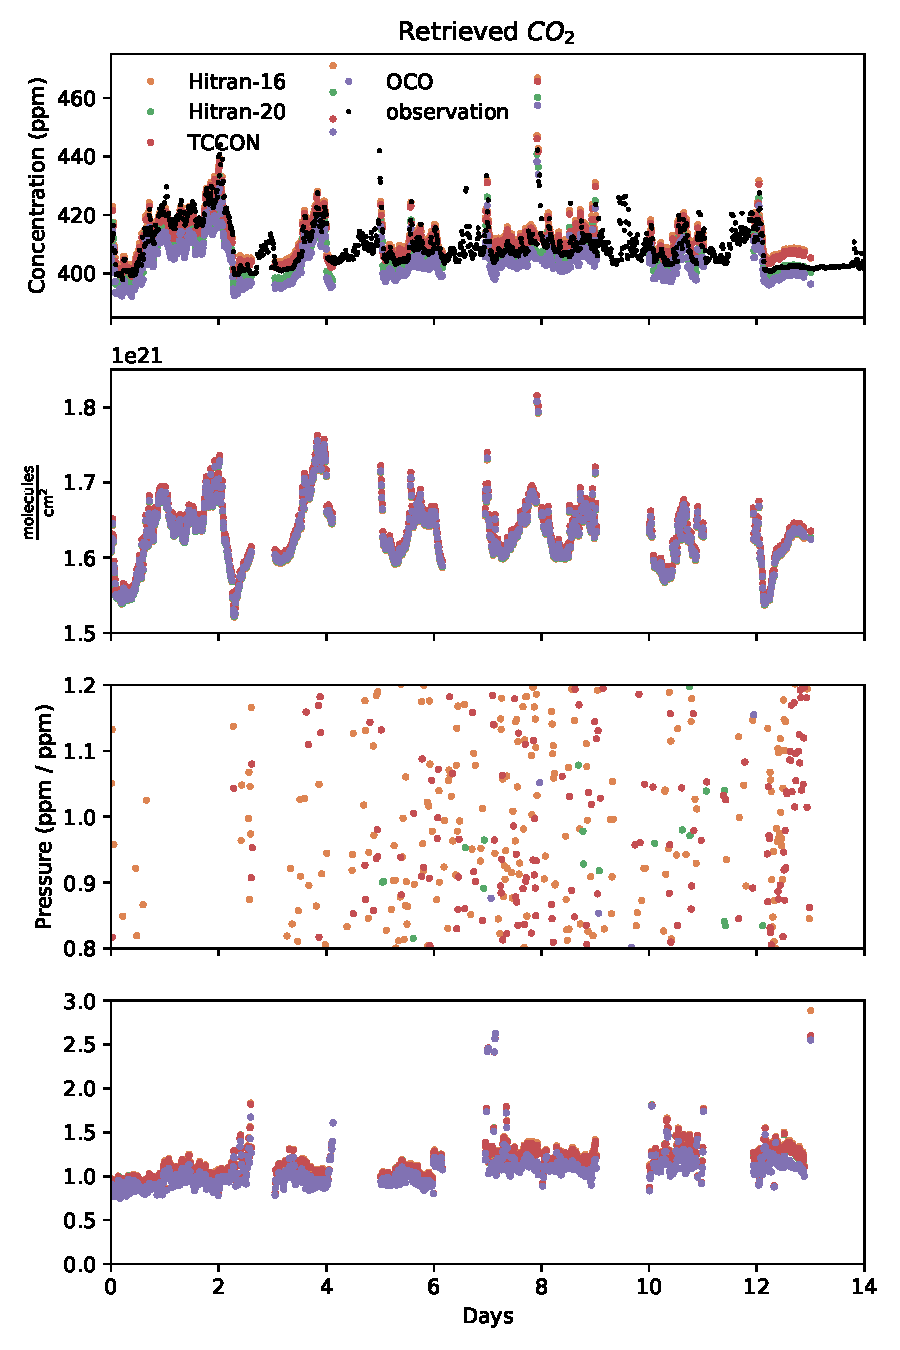
\includegraphics{co2_timeseries.pdf}
  \caption{Retrieved CO$_2$ concentrations with line-lists outlined in Table \ref{tab:1} from our DCS field deployment in Boulder, Colorado, USA over a two week period. From top to bottom, the panels show CO$_2$ concentrations, column densities, relative errors, and reduced $\chi^2$ statistic. }
  \label{fig:co2_timeseries}
\end{figure}



On the other hand, there is considerable disagreement for retrieved methane. Methane’s spectroscopy is continuously evolving (Collins et al, 2018; Myer et al, 2016). Fig. \ref{fig:ch4_timeseries} shows the retrieved methane time-series. Methane’s daily peak is ~200\,pbb above background concentrations. Although less than the CO$_2$ diurnal cycle, methane still exhibits a diurnal cycle, which is driven by boundary layer height and urban emissions in Boulder. CO$_2$ emissions exhibit a more pronounced diurnal cycle, because the sources of CO$_2$, such as vehicle traffic and electricity production, are diurnally varying (Waxman et al, 2018).

We used the Hitran 2008, 2016, and 2020 line-lists , in addition to the TCCON line-list, to retrieve methane concentrations. In contrast to CO$_2$, the methane concentrations can vary by up to xx pbb, which is due to spectroscopic errors. These errors in pressure and temperature-dependent spectroscopic parameters can induce errors in not only the methane column amount, but also the dry air column density, affecting the overall methane concentrations.

Fig. \ref{fig:ch4_timeseries}C shows the ratio between the retrieved methane from the DCS and the measured concentrations from the Picarro instrument. In contrast to CO$_2$, this ratio for methane exhibits a much larger range, from ~0.93 to ~1.07, resulting in a 7\% disagreement in methane concentrations.

\begin{figure}
  \centering
  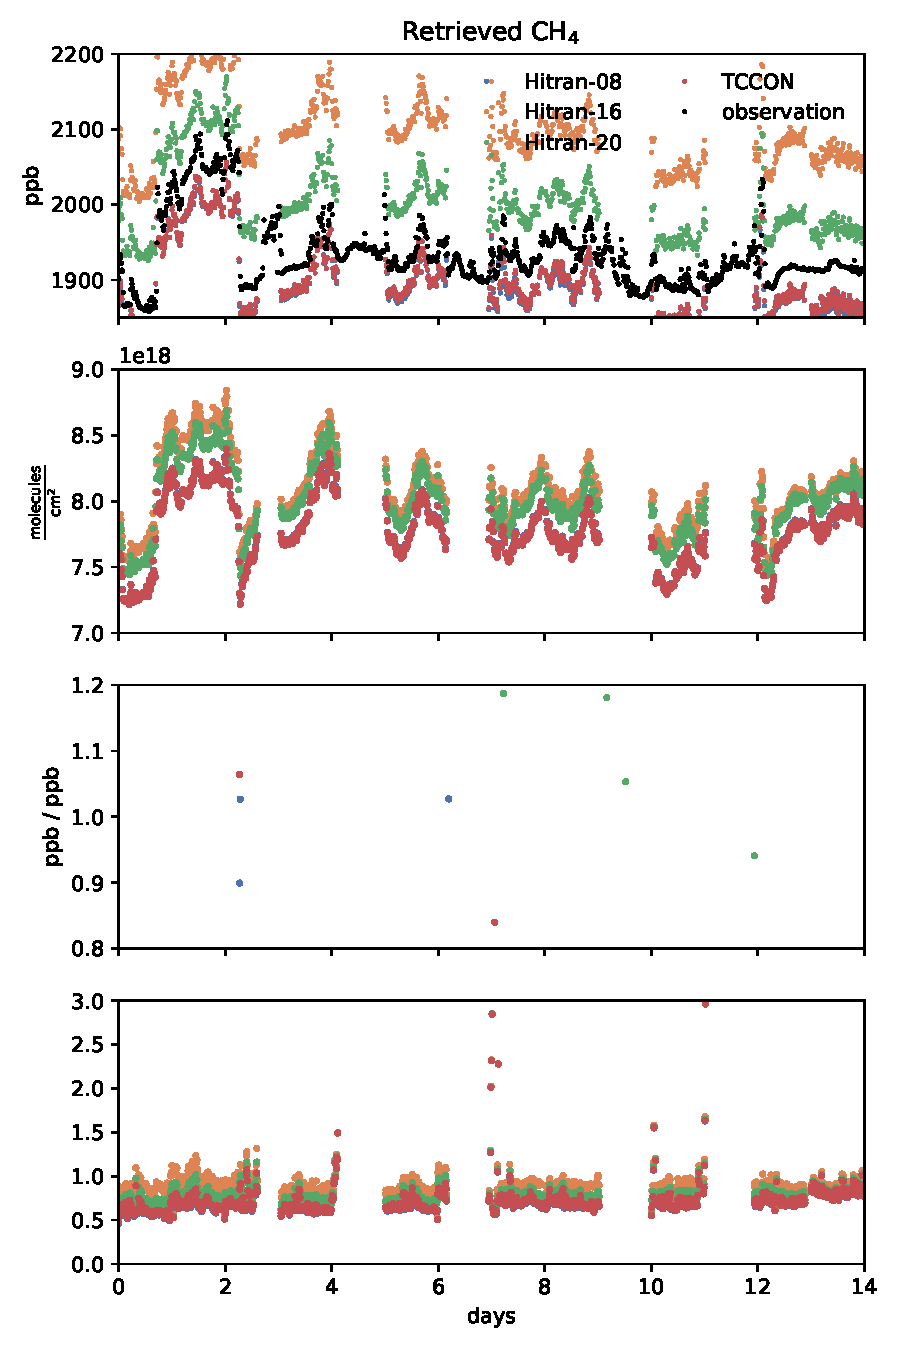
\includegraphics{ch4_timeseries.pdf}
  \caption{Retrieved CH$_4$ from our DCS field-deployment. The figure is arranged as in Fig. \ref{fig:co2_timeseries}.}
  \label{fig:ch4_timeseries}
\end{figure}

\begin{figure}
  \centering
  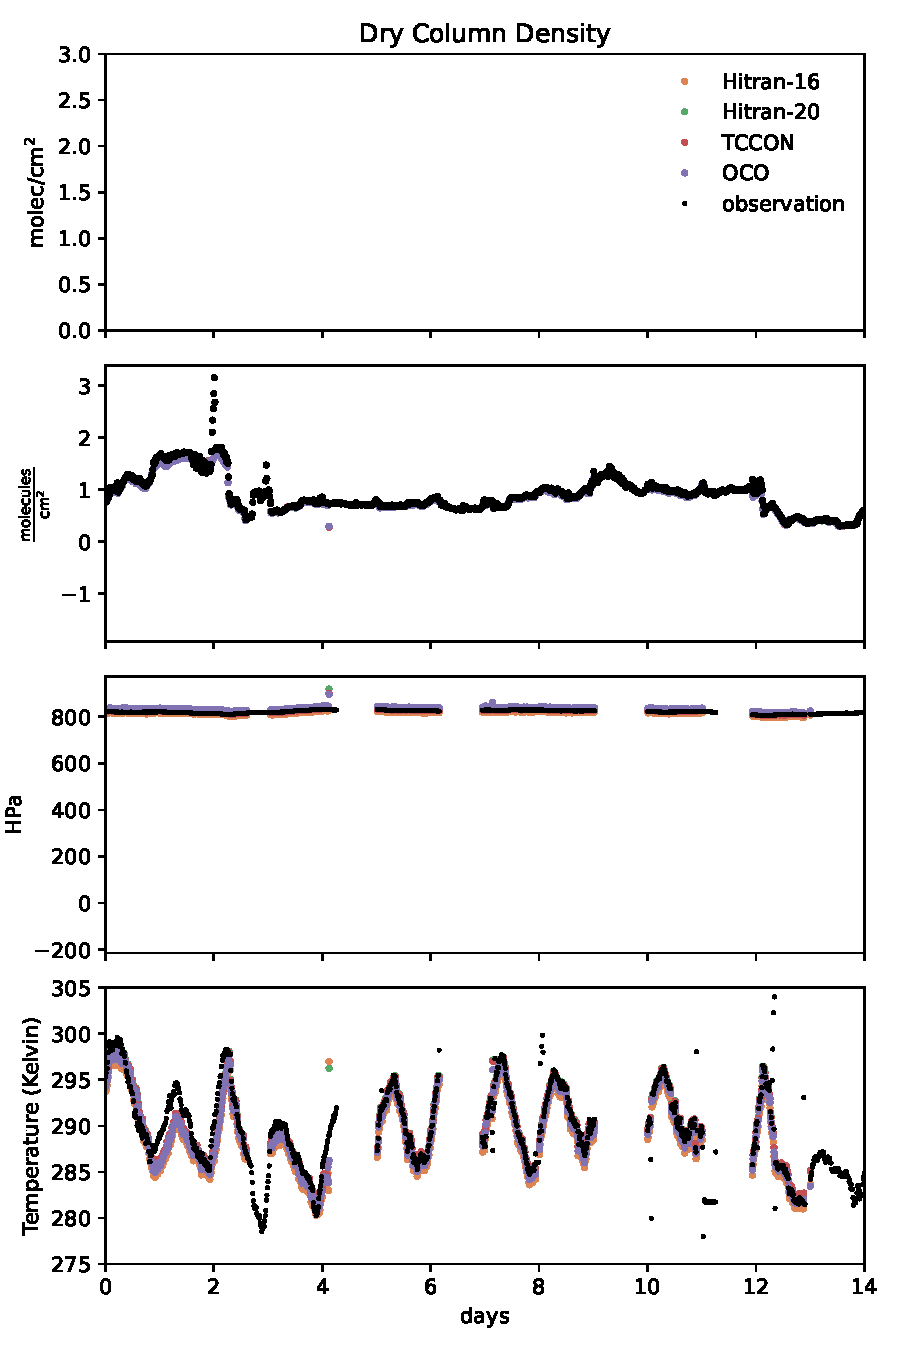
\includegraphics{vcd_timeseries.pdf}
  \caption{Retrieved variables required to calculate the dry column density ($dry_{cd}$). This includes, from top to bottom, dry air column density, water vapor concentration, pressure, and temperature. These variables were retrieved over the CO$_2$ window (6180-6260\,cm$^{-1}$).}
  \label{fig:vcd_timeseries}
\end{figure}

\subsection{Tracing error sources from field retrievals}

\begin{table}
  \centering
  \begin{tabular}{| c | c | c | c | c |}
    Ch$_4$ Correlations & & & \\
    Variable & Hitran 2008 & Hitran 2016 & Hitran 2020 & TCCON \\
    \hline 
    H$_2$O amount & & & \\
    H$_2$O error & & & & \\
    pressure error & & & & \\
    temperature error & & & & \\
    \hline
    CO$_2$ correlations & & & & \\
        H$_2$O amount & & & \\
    H$_2$O error & & & & \\
    pressure error & & & & \\
    temperature error & & & & \\
    \hline

  \end{tabular}
  \caption{Error correlations for our retrievels from the field-deployed DCS. The errors were calculated relative to the Picarro instrument.}
  \label{tab:2}
\end{table}
In order to trace the error sources, we plotted the relative ghg concentrations error as a function of other parameters of interest. They include relative pressure error, retrieved water vapor columns, and relative water vapor error. The relative errors were calculated by computing the percent difference of the retrieved variable compared to the reference measurement taken by the Picarro, pressure, and temperature sensors on the nearby tower. Figs xx and Table xx shows these results. 

For C$_O2$, we find that there are weak correlations when correlating error terms. The relative error correlations between CO$_2$ and pressure range from 0.02, which is from OCO, to 0.14, which are from the Hitran 2016 and 2020 line-lists. Water vapor seems to have the strongest correlation, which ranges between 0.16 to 0.20. 

On the other hand, we find much stronger relationships for methane. From Fig. xx, we can see that there is some correlation between the methane and water vapor relative errors, with a correlation of about 0.49. This indicates that errors in retrieving methane and water are linked. We can trace the source of this error to the pressure retrieval, which has a correlation of -0.33. A negative correlation indicates that high biases in pressure are leading to low bias in retrieved methane. This negative correlation increases when looking at Hitran 2016, which goes up to -0.59, while Hitran 2020 goes back to -0.41. this points to errors from pressure broadening parameters and water vapor spectroscopy aliasing onto the retrieved column.

\subsection{Comparing spectra from different line-lists }

\begin{figure}
  \centering
  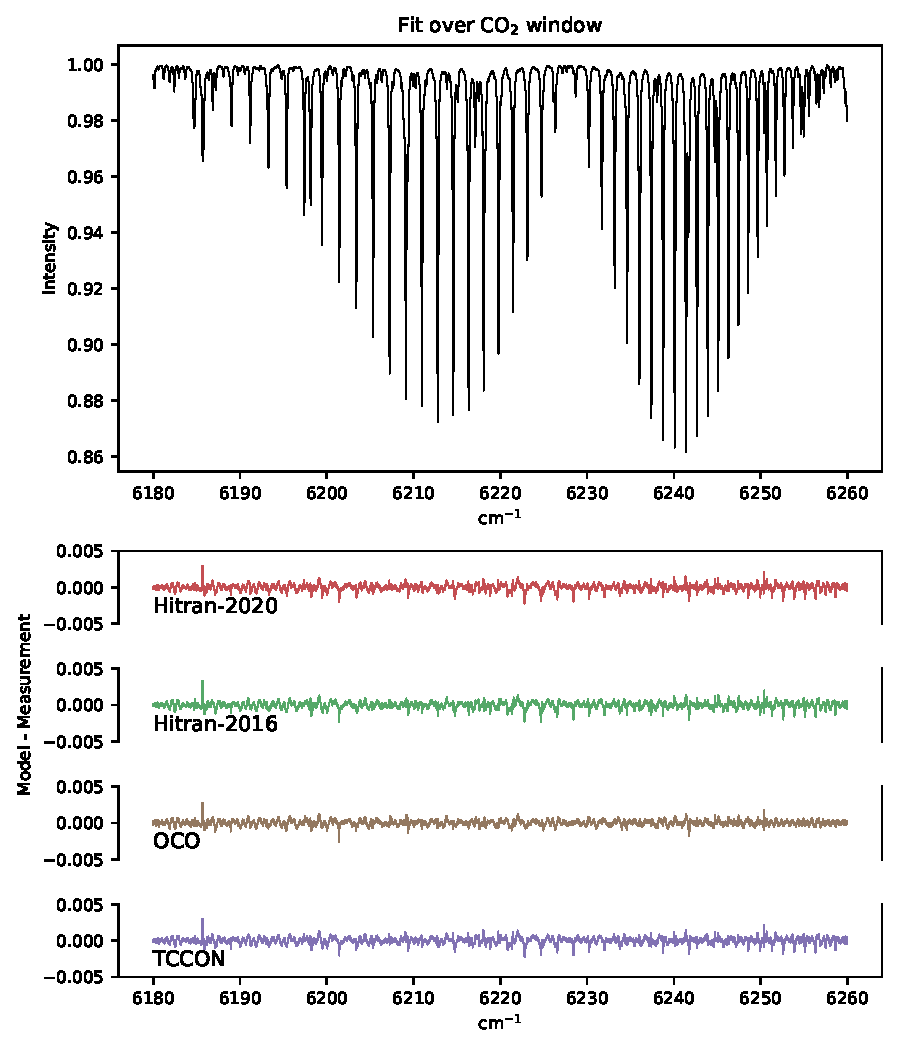
\includegraphics{co2_fit.pdf}
  \caption{DCS Absorption spectrum (top) over the CO$_2$ retrieval window (6180-6260\,cm$^{-1}$). The bottom panel shows modelled residuals from the OCO, Hitran 2016, Hitran 2020, and TCCON line-lists, as outlined in Table \ref{tab:1}. }
  \label{fig:co2_spectrum}
\end{figure}
We can examine the accuracy of the CO$_2$ and methane spectroscopy by looking at the spectral residuals  of our retrieval’s  and comparing them to the measured DCS spectrum. Fig. \ref{fig:co2_spectrum} shows the transmission spectrum, which is the measured transmission divided by the instrument baseline. The data shown in Figs \ref{fig:co2_spectrum} and \ref{fig:ch4_spectrum} are obtained from averaging the spectra over a 24 hour period on 21 September, 2016. Spectra were averaged in order to minimize random noise so that individual absorption features can be closely inspected.

In both Figs. {fig:co2_spectrum} and \ref{fig:ch4_spectrum}, we can see that the residuals between the model and measured spectra only differ by 1e-3, indicating a good model fit to the measured spectra. The root mean squared error for these are xx over the methane window and xx over the CO$_2$ window.

The CO$_2$ window, which ranges between 6180 and 6260\,cm$^{-1}$, is also observed by other instruments, such as SCIAMACHY, OCO, and TCCON. We can see from the spectral residuals in Fig XB that OCO performs best, with a chi2 of xx and rmsd of xx. TCCON also performs well with a Chi2 of xx and rmsd of xxx. We also see that there is not much difference among the fits for different Hitran editions, with chi2 ranging from xx to xx and rmsd ranging from xx to xx.

Although there is not a significant difference between each of these spectral residuals, OCO does perform best. This is due to the additional physical processes accounted for in the OCO spectroscopy, which includes line-mixing and other processes beyond just pressure and temperature broadening. In a retrieval with pressure and temperature, incorporating the additional processes makes calculations of the dry air column amount more accurate [Hartmann et al., 2008; Long et al., 2022; Malina et al, 2022].

\begin{figure}
  \centering
  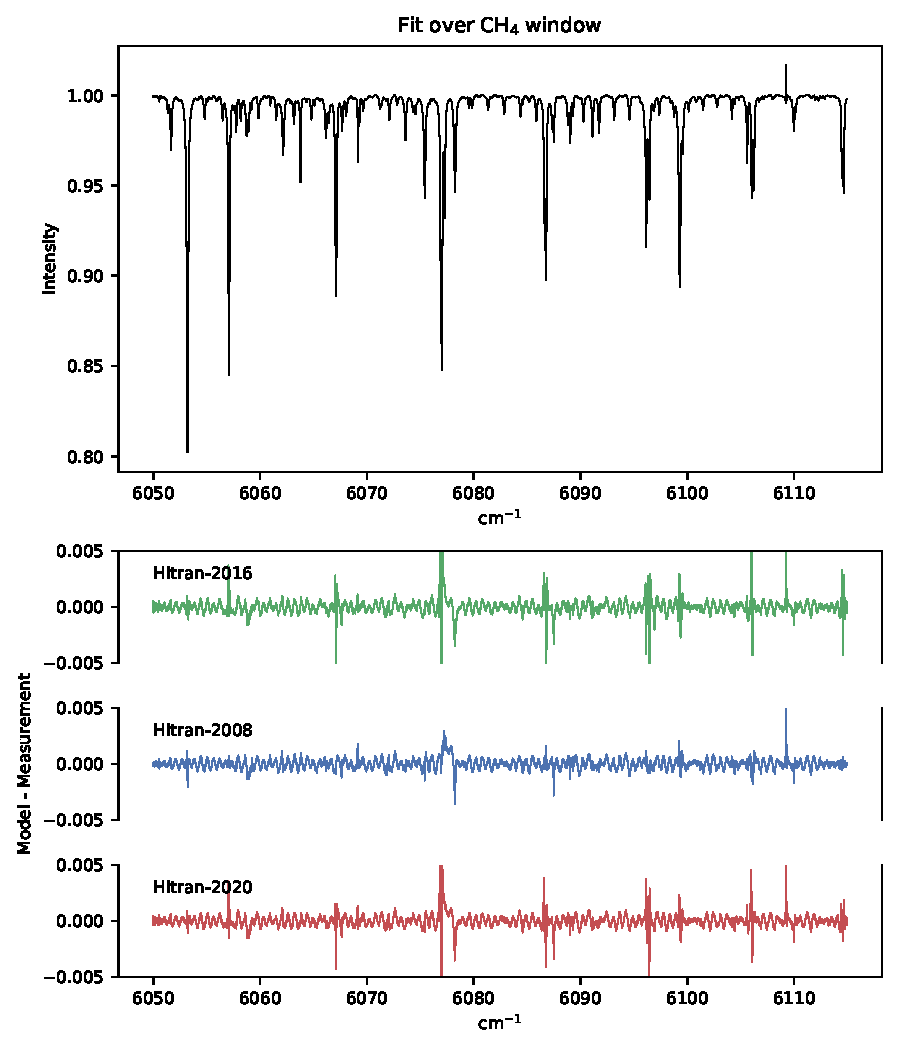
\includegraphics{ch4_fit.pdf}
  \caption{DCS absorption spectrum over the CH$_4$ fitting window (6050-6115\,cm$^{-1}$), on top. The bottom panel shows the residuals with modelled spectra using the Hitran 2008, Hitran 2016, Hitran 2020, and TCCON line-lists.}
  \label{fig:ch4_spectrum}
\end{figure}

In contrast to CO$_2$, Fig XB shows a large difference in the methane residuals. We can see that Hitran 2008 has the best fit, with a chi2 of xx and rmsd of xx. TCCON performs similarly to Hitran 2008 (chi2=xx and rmsd=xx), because TCCON obtained their parameters from Hitran 2008. Interestingly, the worst performing spectroscopy comes from Hitran 2016 with a chi2 of xx and rmsd of xx. The subsequent update to Hitran 2020 improved the fits to be on par with Hitran 2008 with a chi2 of xx and rmsd of xx.

The Merlin mission will be analyzing the R6 methane transition. Fig. \ref{fig:ch4_spectrum_r6} shows a zoom into the R6 transition between 6076 to 6079 wavenumbers. We find that here, there are systematic residuals in all the line-lists. This indicates that there are both parameter and model errors in this region. Several studies have more closely examined this specific transition e.g., citations. They find that accounting for additional processes, such as line-mixing and collision induced absorption, through the Hartman Tran Profile improves the fits to xx\%. Since the DCS has a broader spectral range, similar analyses and parameter optimizations should be performed over additional transitions over the DCS ranges in order to obtain the most accurate modeled absorptions of methane. 

\begin{figure}
  \centering
  includegraphics{ch4_fit_R6.pdf}
  \caption{Zoom into the CH$_4$ R6 transition, which will be observed by the Merlin Mission. }
  \label{fig:ch4_spectrum_r6}
\end{figure}
Methane spectroscopy is particularly challenging, because of the manifolds in vibrational and rotational transitions, which creates a blend of overlapping absorption lines, resulting in line-shape asymmetries and additional difficulty in modeling the line-shape. The Voigt Profile does not account for these more complex processes. However, we find that errors that arise from the complexity of the line-shape is outweighed by the errors in the line-shape parameters themselves. This is in agreement with Reiker et al (2014). Calculating more accurate spectroscopic parameters for methane is an on-going effort, and we find that it is necessary in order to achieve highly accurate methane measurements with the DCS.

\section{Synthetic Retrieval Experiments}
\subsection{Pressure errors cause disagreements among different line-lists}

\begin{figure}
  \centering
  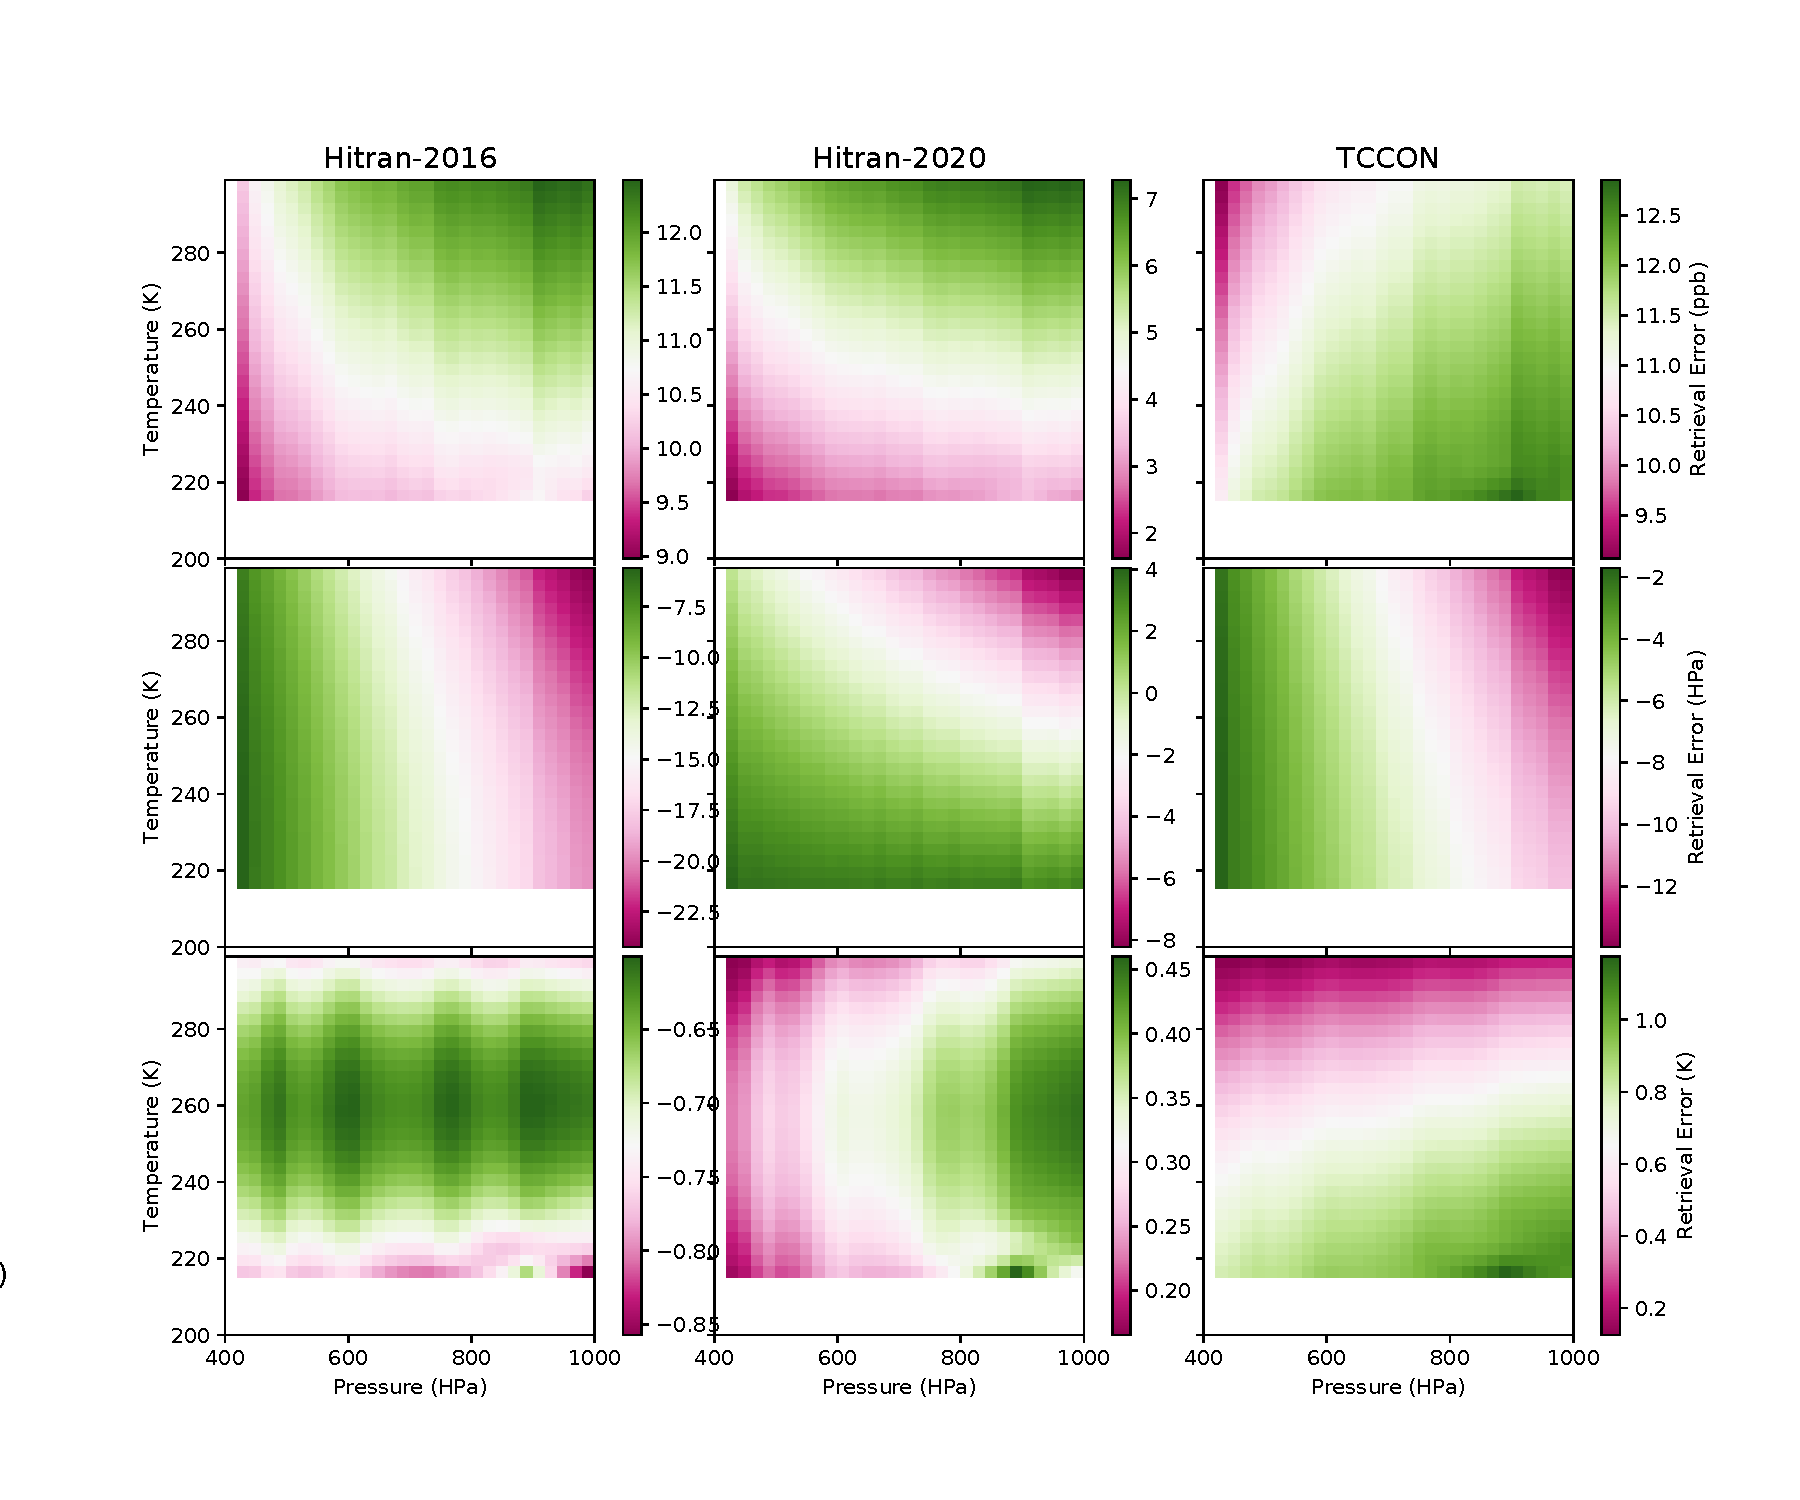
\includegraphics{heatmap_co2.pdf}
  \caption{Retrieval errors from our $CO$_2$ synthetic retrieval experiments. The 'true spectra' were generated wie OCO line-list.}
  \label{fig:co2_retrieval_error}
\end{figure}
We performed synthetic retrieval’s In order to find the disagreement among the line-lists used in this study. Synthetic measurements were generated using the most accurate line-lists for the species: OCO line-list for CO$_2$, TCCON for water vapor, and Hitran 2008 for methane. We generated the synthetic spectra over a range of pressures and temperatures. Then, we performed the retrieval with different line-lists in order to calculate the retrieval error. In our retrievals, we also fitted for pressure and temperature, which enables us to calculate how much the retrieval error of our greenhouse gas concentrations varies with pressure and temperature. Figs \ref{fig:co2_synthetic_retrieval} and \ref{ch4_synthetic_retrieval} display our results.

For methane, we find that errors are large, maxing out at xx ppb at p=xx and T=xx for Hitran 2016 and xx for Hitran 2020. From our synthetic retrievals, we can see that temperature errors are minimal, varying by about 1 degree, while the retrieval error for pressure can be up to xx HPa. This indicates that errors in methane are largely due to errors in modeling pressure effects, which can be traced to either model error or parameter error.

Talk about how these variable bites are a function of pressure and temperature and where the biases is the highest

\begin{figure}
  \centering
  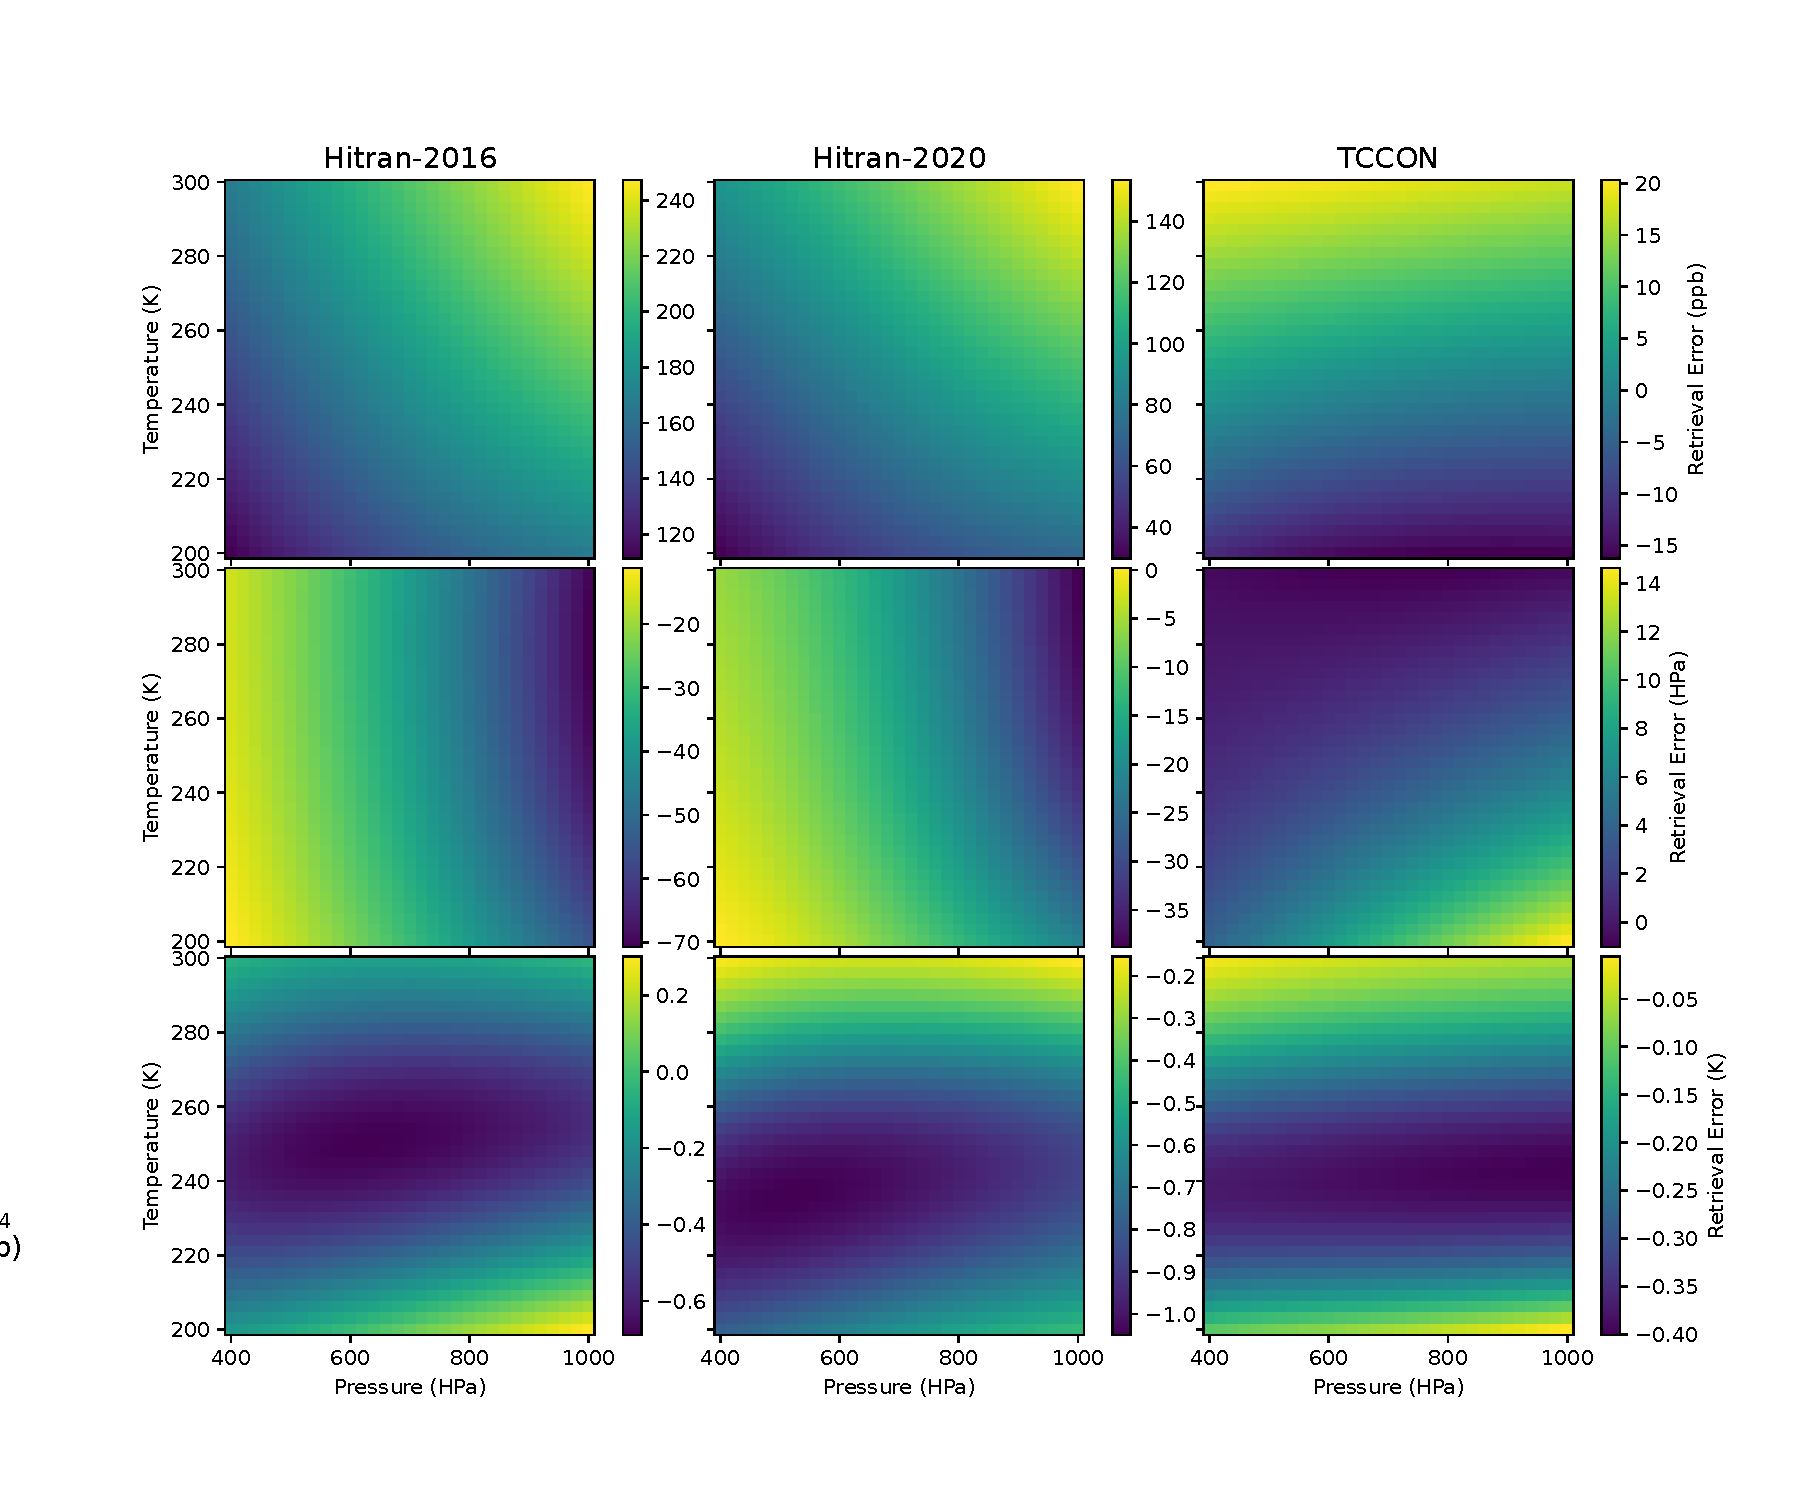
\includegraphics{heatmap_ch4.pdf}
  \caption{Retrieval error for CH$_4$ synthetic retrievals. The 'true spectra' were generated with Hitran 2008.}
  \label{fig:ch4_synthetic_retrieval}
\end{figure}

\subsection{Quantifying effects of errors in pressure broadening}
We can further quantify this with a numerical experiment, where we perturb the pressure broadening parameters. In this case, we perturbed the temperature dependence of pressure broadening, called n\_air in Hitran,  by 5\%, which is within error of that parameter.

Fig. \ref{fig:param_pert} shows the results of our parameter broadening experiment. At temperatures close to the reference temperature of 298 K, the retrieval error is minimal, at around 20 ppb, and this is independent of pressure. the retrieval error increases farther from the reference temperature, and it is maximized at very low temperatures and peak at around 45 ppb. This relationship is because of xx reasons. 

The biases in this perturbation experiment are also pressure and temperature dependent. describe the relationship with pressure and temperature. 

In general, this experiment shows two things. First of all, the biases incurred from small errors in these parameters can be substantial. Our results show that a 5\% perturbation in this parameter can incur up to a 2.5\% error in the retrieved concentrations. Secondly, biases in retrieved greenhouse gas concentrations, specifically methane, are nonlinear and depend on pressure and temperature. The biases are maximized at lower temperatures. Given these results, more certainty is needed for parameters affecting pressure broadening in methane spectroscopy. This is important for fully realizing the technological potential of DCS to obtain laboratory-level accurate greenhouse gas measurements in the field and for the ability of DCS to measure vertical ghg gradients in the atmosphere – a future DCS application.
\begin{figure}
  \centering
  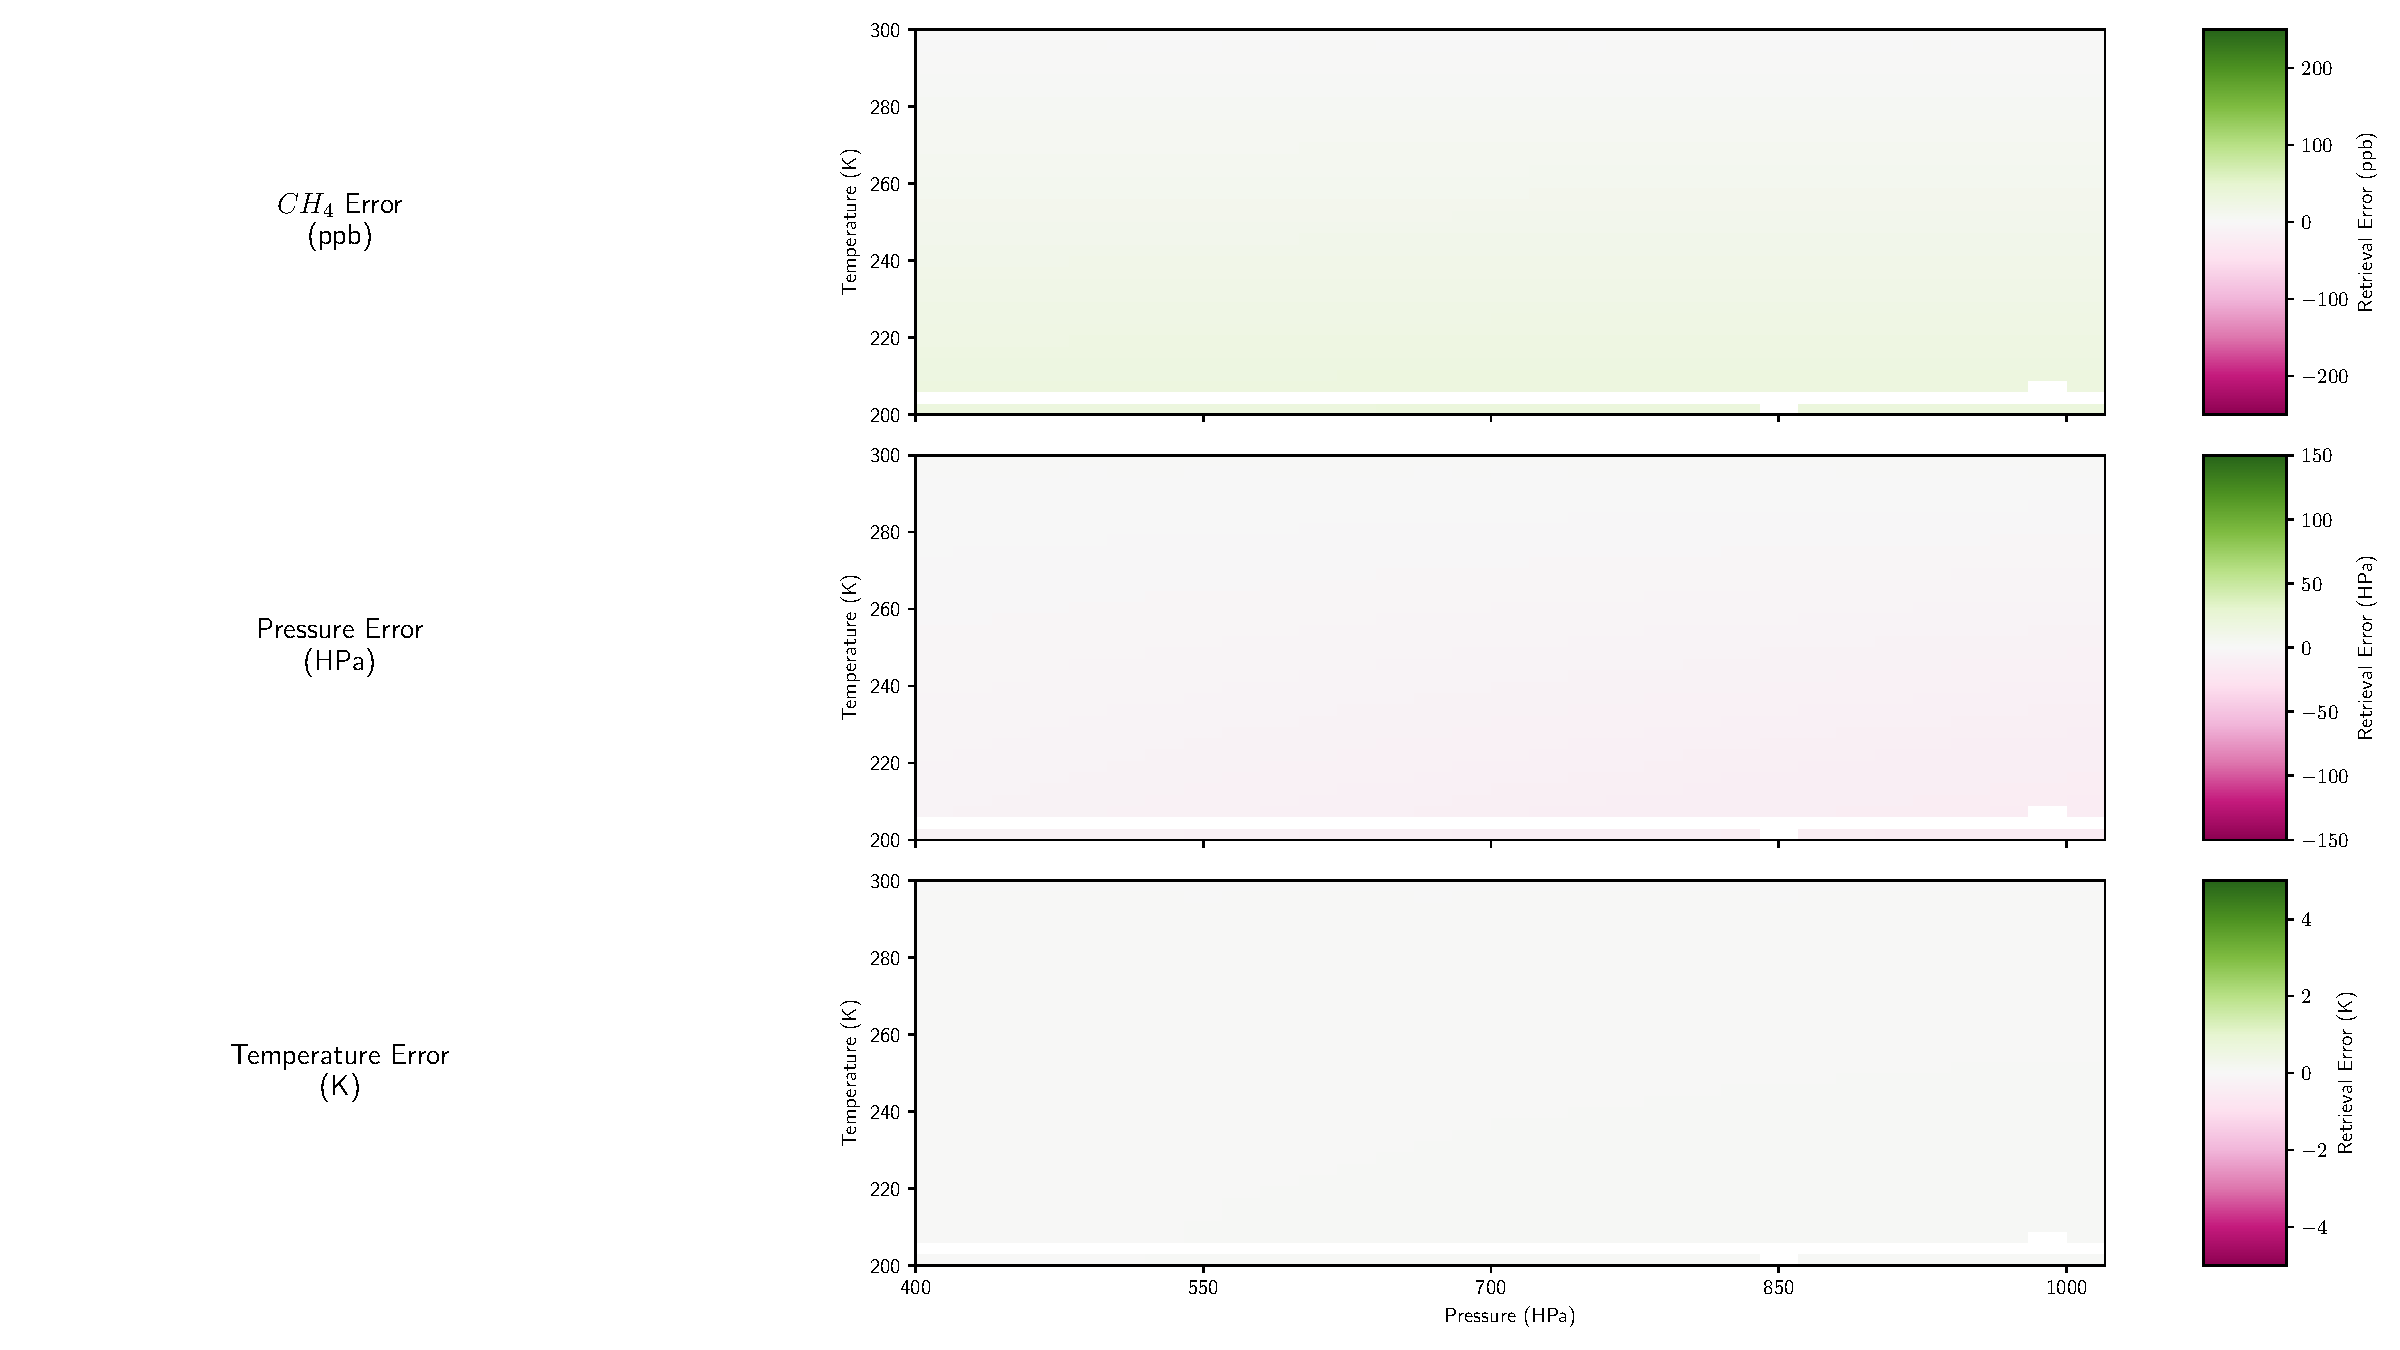
\includegraphics{ch4_params_pert.pdf}
  \caption{Synthetic retrieval of CH$_4$ with a 5\% perturbation to the temperature dependence on pressure broadening.}
  \label{fig:param_pert}
\end{figure}
\section{Vertical Profile Retrievals}
\subsection{Measuring Vertical Gradient’s: A DCS Application }
Measuring vertical ghg gradients is a future DCS application. The long-range, open-path, and absolute stability of the active light source enables highly accurate spectra to be measured. The DCS would be on the ground, aimed at a balloon with a mounted retro-reflector, and the return-signal would be measured on the ground. The high spectral sampling of the DCS would enable precise interrogation of narrower absorption features characteristic of the upper atmosphere, and the absolute frequency stability would enable accurate measurements of absorption features through spectral averaging. This makes DCS an excellent candidate for ground-based vertical profile measurements.

Vertical profile measurements will provide additional constraints on how greenhouse gases are transported throughout the atmosphere and top-down ghg flux inversions. Moreover, there is considerable disagreement in ghg vertical gradients in chemical transport models. currently, ghg vertical gradients are measured through flasks from air and balloon flights and the NOAA Air Core Program [Karion]. The DCS can augment these measurements with more numerous vertical profile measurements in a future network. 

There has been recent work on developing vertical profile retrievals from ground-based spectral measurements measured by TCCON (e.g., Kuai et al, 2014, Roche et al, 2021). One of the major error terms was uncertainties in the instrument’s line-shape (Roche et al, 2021), which requires constant calibration (Wunsch  et al, 2011). The DCS can provide ground-based spectral measurements free from the distortions of an instrument line-shape. 

Here, we quantify the additional information that a ground-based DCS vertical profile retrieval can provide. Through calculations of the Degrees of Freedom, which arises from the information content of the retrieval, we can calculate the number of layers that can be retrieved from a vertical profile retrieval. In order to ascertain the importance of pressure and temperature broadening effects, we also quantify the information that variations in pressure and temperature in the atmosphere provides by assuming an isothermal and isobaric atmosphere. In these synthetic experiments, we assume that the DCS is pointing straight up at a balloon at an altitude of 10 km, so the round-trip path length is 20 km.

\subsection{Retrieval Algorithm and analysis Methods }
Our vertical profile retrieval algorithm employs the Optimal Estimation Method developed by Rogers 2000. This Bayesian method is necessary, because the problem is ill-posed. Incorporating prior information about the atmospheric state then transforms the cost function into the following equation:

j(x) =

In equation xx, there are two terms being minimized. the first term is the misfit between the observed and modeled instrument measurement, which is the same as Section 2. The second term is the misfit between the prior ( or initial state) and the retrieved state (the solution). Both terms are weighted by an error covariance matrix. The measurement misfit is weighted by the measurement covariance matrix, which contains the instrument errors. The misfit of the prior and retrieved state is weighted by the prior error covariance, which contains the uncertainties for each state variable in the main diagonal elements and the correlation between the variables in the off-diagonal elements. Physically, the off-diagonal terms of the prior error covariance matrix are the correlation between different layers, and we set the correlation length scale to 50 HPa. The off-diagonal elements are calculated using the following equation:

Since the problem is nonlinear, the state vector, x, needs to be iteratively updated, which is calculated by the following equations:

here, Gamma is a Tikhonov regularization parameter that dictates the importance of the prior knowledge and changes the step-size between each iteration. We enable gamma to adapt to the linearity of the problem at each step, decreasing at near linear states and increasing farther away from linearity.

For the forward model, we also employ the Lambert-Beer law over multiple layers:

here, $tau\_i$ is the optical depth of layer i and  $\sigma_{ij}$ is the cross-section for layer i and species j. Since there are additional layers, the problem becomes more nonlinear, so we linearize the problem by solving it in log-space. The forward model then becomes the following:

\subsection{High spectral sampling of the DCS enables more retrieved layers }
We developed a simulation of DCS measurements in a vertical profile setting for a standard atmosphere. Vertical profile retrievals can be assessed by the Degrees of Freedom (DOF) of the retrieval. The DOF corresponds to the number of atmospheric layers that can be inferred, which is calculated using the following equations:

explain the terms in the equations
Table 2 shows the DOF for each the retrieved species. We get about 4 DOF for CO$_2$, 3 for methane, and about 4.5 for water vapor. This is in comparison to a TCCON retrieval, which contains xx for CO$_2$ and xx for methane [citations]. 


\subsection{Quantifying retrieved information from pressure versus temperature }
\begin{table}
  \centering
  \begin{tabular}{| c | c | c | c |}
    species & standard & isobaric & isothermal \\
    \hline
    CH$_4$ & & & \\
    CO$_2$ & & & \\
    H$_2$O & & & \\
    \hline
  \end{tabular}
  \caption{Degrees of Freedom from our synthetic vertical profile experiments.}
  \label{tab:3}
\end{table}
We also compute the information that atmospheric variations in pressure and temperature contribute to a vertical profile retrieval. To do this, we model the transmission and absorption through an isothermal and isobaric atmosphere. Table \ref{tab:3} displays our results. We find that for methane, the DOF for pressure variations is xx while temperature is xx. For CO$_2$, pressure contributes xx DOF, while temperature contributes xx. finally, for water vapor, pressure contributes xx, while temperature variations contribute xx. Note that the sum of the pressure and temperature DOF does not equal the total DOF for a standard atmosphere, because the information contained in pressure and temperature variations are not orthogonal. 

In general, pressure variations (the isothermal atmosphere simulations) contribute more information. This is due to the fact that the dynamic range for pressure is higher than that of temperature in an atmospheric profile. Overall, this also underlines the importance of calculating accurate pressure broadening effects of ghg spectra, which is also emphasized in Roche et al (2021).



\section{Summary and Discussion}
Dual Comb spectroscopy brings laboratory-level accurate spectroscopy directly into the field. Its absolute frequency stability and high spectral sampling enables high-resolution interrogation of molecular absorption features. However, we showed that limitations of the spectroscopic parameters of ghgs, mainly methane and water vapor, prevent highly accurate retrievals of greenhouse gas concentrations. With field data, we found that errors in methane spectroscopy can lead to more than a 5\% disagreement in retrieved methane concentrations, while CO$_2$ was xx\%.

We found that these errors are correlated with pressure errors and water vapor errors, which affect the column density and alias on to the retrieved concentrations. Our numerical experiment, where we calculated the retrieval error as a function of pressure and temperature, indicate that a large portion of the error is due to errors in pressure broadening parameters, while the errors from temperature effects are minimal. Our numerical perturbation experiment showed that an only 5\% error in the temperature dependence on pressure broadening can actually incur a 2.5\% in retrieved methane, and the bias is also dependent on pressure and temperature.

We also developed a vertical profile retrieval algorithm for the DCS, which is a future application. From these experiments, we find that the high spectral resolution of the DCS can enable additional layers to be retrieved. mOreover, the frequency stability of the DCS also enables higher signal to noise ratios by time-averaging free from instrument drift . We quantified the information that atmospheric pressure and temperature variations bring, and our synthetic isobaric and isothermal atmosphere tests show that a majority of the information comes from variations in atmospheric pressure. This underlines the importance of obtaining more accurate pressure broadening parameters to model these effects.

the dependence of the biases to pressure and temperature prevent simple rescaling, and since the errors are not random, they cannot be simply averaged out. this variable error underlines the necessity of improved ghg spectroscopic parameters. Overall, the DCS will enable highly accurate greenhouse gas measurements from the surface and throughout the atmosphere. However, improvements to  ghg spectroscopy should be made in order for DCS measurements to obtain the 0.1\% accuracy necessary for ghg monitoring. 




\conclusions  %% \conclusions[modified heading if necessary]
Dual Comb Spectroscopy has the potential of augmenting our greenhouse gas observation network by bringing laboratory-level accurate spectroscopy directly into the field. To aid in this application, we developed a retrieval algorithm that separates the effects of pressure and temperature from the retrieved greenhouse gas amounts by utilizing the high spectral resolution of the DCS. We found that while there do exist spectroscopic errors in methane and CO$_2$, it is important to properly model the effects of pressure-broadening on ghgs. We also found that the high spectral sampling of the DCS enables direct retrieval of pressure and temperature from only the shape of the measured absorption cross-sections. In order to have the DCS achieve the 0.1\% accuracy necessary for monitoring ambient ghgs and their trends, additional laboratory work should be done to measure and quantify the spectroscopic parameters of methane. The DCS would also be an ideal instrument for obtaining spectroscopic parameters, given that it is free from the distorting effects of the instrument line-shape.

DCS is a novel method of measuring greenhouse gases. By employing the time-keeping stability of the instrument, we can now bring laboratory-level accurate measurements directly into the field. However, without ancillary measurements to quantify the dry air column, the accuracy of the DCS retrieval is not limited by the instrument, but by the accuracy of greenhouse gas spectroscopy itself.
%% The following commands are for the statements about the availability of data sets and/or software code corresponding to the manuscript.
%% It is strongly recommended to make use of these sections in case data sets and/or software code have been part of your research the article is based on.

\codeavailability{TEXT} %% use this section when having only software code available


\dataavailability{TEXT} %% use this section when having only data sets available


\codedataavailability{TEXT} %% use this section when having data sets and software code available


\sampleavailability{TEXT} %% use this section when having geoscientific samples available


\videosupplement{TEXT} %% use this section when having video supplements available


\appendix
\section{}    %% Appendix A

\subsection{}     %% Appendix A1, A2, etc.


\noappendix       %% use this to mark the end of the appendix section. Otherwise the figures might be numbered incorrectly (e.g. 10 instead of 1).

%% Regarding figures and tables in appendices, the following two options are possible depending on your general handling of figures and tables in the manuscript environment:

%% Option 1: If you sorted all figures and tables into the sections of the text, please also sort the appendix figures and appendix tables into the respective appendix sections.
%% They will be correctly named automatically.

%% Option 2: If you put all figures after the reference list, please insert appendix tables and figures after the normal tables and figures.
%% To rename them correctly to A1, A2, etc., please add the following commands in front of them:

\appendixfigures  %% needs to be added in front of appendix figures

\appendixtables   %% needs to be added in front of appendix tables

%% Please add \clearpage between each table and/or figure. Further guidelines on figures and tables can be found below.



\authorcontribution{TEXT} %% this section is mandatory

\competinginterests{TEXT} %% this section is mandatory even if you declare that no competing interests are present

\disclaimer{TEXT} %% optional section

\begin{acknowledgements}
TEXT
\end{acknowledgements}




%% REFERENCES

%% The reference list is compiled as follows:

\begin{thebibliography}{}

\bibitem[AUTHOR(YEAR)]{LABEL1}
REFERENCE 1

\bibitem[AUTHOR(YEAR)]{LABEL2}
REFERENCE 2

\end{thebibliography}

%% Since the Copernicus LaTeX package includes the BibTeX style file copernicus.bst,
%% authors experienced with BibTeX only have to include the following two lines:
%%
%% \bibliographystyle{copernicus}
%% \bibliography{example.bib}
%%
%% URLs and DOIs can be entered in your BibTeX file as:
%%
%% URL = {http://www.xyz.org/~jones/idx_g.htm}
%% DOI = {10.5194/xyz}


%% LITERATURE CITATIONS
%%
%% command                        & example result
%% \citet{jones90}|               & Jones et al. (1990)
%% \citep{jones90}|               & (Jones et al., 1990)
%% \citep{jones90,jones93}|       & (Jones et al., 1990, 1993)
%% \citep[p.~32]{jones90}|        & (Jones et al., 1990, p.~32)
%% \citep[e.g.,][]{jones90}|      & (e.g., Jones et al., 1990)
%% \citep[e.g.,][p.~32]{jones90}| & (e.g., Jones et al., 1990, p.~32)
%% \citeauthor{jones90}|          & Jones et al.
%% \citeyear{jones90}|            & 1990



%% FIGURES

%% When figures and tables are placed at the end of the MS (article in one-column style), please add \clearpage
%% between bibliography and first table and/or figure as well as between each table and/or figure.

% The figure files should be labelled correctly with Arabic numerals (e.g. fig01.jpg, fig02.png).


%% ONE-COLUMN FIGURES

%%f
%\begin{figure}[t]
%\includegraphics[width=8.3cm]{FILE NAME}
%\caption{TEXT}
%\end{figure}
%
%%% TWO-COLUMN FIGURES
%
%%f
%\begin{figure*}[t]
%\includegraphics[width=12cm]{FILE NAME}
%\caption{TEXT}
%\end{figure*}
%
%
%%% TABLES
%%%
%%% The different columns must be seperated with a & command and should
%%% end with \\ to identify the column brake.
%
%%% ONE-COLUMN TABLE
%
%%t
%\begin{table}[t]
%\caption{TEXT}
%\begin{tabular}{column = lcr}
%\tophline
%
%\middlehline
%
%\bottomhline
%\end{tabular}
%\belowtable{} % Table Footnotes
%\end{table}
%
%%% TWO-COLUMN TABLE
%
%%t
%\begin{table*}[t]
%\caption{TEXT}
%\begin{tabular}{column = lcr}
%\tophline
%
%\middlehline
%
%\bottomhline
%\end{tabular}
%\belowtable{} % Table Footnotes
%\end{table*}
%
%%% LANDSCAPE TABLE
%
%%t
%\begin{sidewaystable*}[t]
%\caption{TEXT}
%\begin{tabular}{column = lcr}
%\tophline
%
%\middlehline
%
%\bottomhline
%\end{tabular}
%\belowtable{} % Table Footnotes
%\end{sidewaystable*}
%
%
%%% MATHEMATICAL EXPRESSIONS
%
%%% All papers typeset by Copernicus Publications follow the math typesetting regulations
%%% given by the IUPAC Green Book (IUPAC: Quantities, Units and Symbols in Physical Chemistry,
%%% 2nd Edn., Blackwell Science, available at: http://old.iupac.org/publications/books/gbook/green_book_2ed.pdf, 1993).
%%%
%%% Physical quantities/variables are typeset in italic font (t for time, T for Temperature)
%%% Indices which are not defined are typeset in italic font (x, y, z, a, b, c)
%%% Items/objects which are defined are typeset in roman font (Car A, Car B)
%%% Descriptions/specifications which are defined by itself are typeset in roman font (abs, rel, ref, tot, net, ice)
%%% Abbreviations from 2 letters are typeset in roman font (RH, LAI)
%%% Vectors are identified in bold italic font using \vec{x}
%%% Matrices are identified in bold roman font
%%% Multiplication signs are typeset using the LaTeX commands \times (for vector products, grids, and exponential notations) or \cdot
%%% The character * should not be applied as mutliplication sign
%
%
%%% EQUATIONS
%
%%% Single-row equation
%
%\begin{equation}
%
%\end{equation}
%
%%% Multiline equation
%
%\begin{align}
%& 3 + 5 = 8\\
%& 3 + 5 = 8\\
%& 3 + 5 = 8
%\end{align}
%
%
%%% MATRICES
%
%\begin{matrix}
%x & y & z\\
%x & y & z\\
%x & y & z\\
%\end{matrix}
%
%
%%% ALGORITHM
%
%\begin{algorithm}
%\caption{...}
%\label{a1}
%\begin{algorithmic}
%...
%\end{algorithmic}
%\end{algorithm}
%
%
%%% CHEMICAL FORMULAS AND REACTIONS
%
%%% For formulas embedded in the text, please use \chem{}
%
%%% The reaction environment creates labels including the letter R, i.e. (R1), (R2), etc.
%
%\begin{reaction}
%%% \rightarrow should be used for normal (one-way) chemical reactions
%%% \rightleftharpoons should be used for equilibria
%%% \leftrightarrow should be used for resonance structures
%\end{reaction}
%
%
%%% PHYSICAL UNITS
%%%
%%% Please use \unit{} and apply the exponential notation


\end{document}
